% Options for packages loaded elsewhere
\PassOptionsToPackage{unicode}{hyperref}
\PassOptionsToPackage{hyphens}{url}
%
\documentclass[
]{article}
\usepackage{lmodern}
\usepackage{amssymb,amsmath}
\usepackage{ifxetex,ifluatex}
\ifnum 0\ifxetex 1\fi\ifluatex 1\fi=0 % if pdftex
  \usepackage[T1]{fontenc}
  \usepackage[utf8]{inputenc}
  \usepackage{textcomp} % provide euro and other symbols
\else % if luatex or xetex
  \usepackage{unicode-math}
  \defaultfontfeatures{Scale=MatchLowercase}
  \defaultfontfeatures[\rmfamily]{Ligatures=TeX,Scale=1}
\fi
% Use upquote if available, for straight quotes in verbatim environments
\IfFileExists{upquote.sty}{\usepackage{upquote}}{}
\IfFileExists{microtype.sty}{% use microtype if available
  \usepackage[]{microtype}
  \UseMicrotypeSet[protrusion]{basicmath} % disable protrusion for tt fonts
}{}
\makeatletter
\@ifundefined{KOMAClassName}{% if non-KOMA class
  \IfFileExists{parskip.sty}{%
    \usepackage{parskip}
  }{% else
    \setlength{\parindent}{0pt}
    \setlength{\parskip}{6pt plus 2pt minus 1pt}}
}{% if KOMA class
  \KOMAoptions{parskip=half}}
\makeatother
\usepackage{xcolor}
\IfFileExists{xurl.sty}{\usepackage{xurl}}{} % add URL line breaks if available
\IfFileExists{bookmark.sty}{\usepackage{bookmark}}{\usepackage{hyperref}}
\hypersetup{
  pdftitle={Membrane Protein: Structure and Stability},
  pdfauthor={Tianyi Shi},
  hidelinks,
  pdfcreator={LaTeX via pandoc}}
\urlstyle{same} % disable monospaced font for URLs
\usepackage[margin=1in]{geometry}
\usepackage{longtable,booktabs}
% Correct order of tables after \paragraph or \subparagraph
\usepackage{etoolbox}
\makeatletter
\patchcmd\longtable{\par}{\if@noskipsec\mbox{}\fi\par}{}{}
\makeatother
% Allow footnotes in longtable head/foot
\IfFileExists{footnotehyper.sty}{\usepackage{footnotehyper}}{\usepackage{footnote}}
\makesavenoteenv{longtable}
\usepackage{graphicx}
\makeatletter
\def\maxwidth{\ifdim\Gin@nat@width>\linewidth\linewidth\else\Gin@nat@width\fi}
\def\maxheight{\ifdim\Gin@nat@height>\textheight\textheight\else\Gin@nat@height\fi}
\makeatother
% Scale images if necessary, so that they will not overflow the page
% margins by default, and it is still possible to overwrite the defaults
% using explicit options in \includegraphics[width, height, ...]{}
\setkeys{Gin}{width=\maxwidth,height=\maxheight,keepaspectratio}
% Set default figure placement to htbp
\makeatletter
\def\fps@figure{htbp}
\makeatother
\setlength{\emergencystretch}{3em} % prevent overfull lines
\providecommand{\tightlist}{%
  \setlength{\itemsep}{0pt}\setlength{\parskip}{0pt}}
\setcounter{secnumdepth}{5}
\ifluatex
  \usepackage{selnolig}  % disable illegal ligatures
\fi

\title{Membrane Protein: Structure and Stability}
\author{Tianyi Shi}
\date{2020-11-12}

\begin{document}
\maketitle

{
\setcounter{tocdepth}{2}
\tableofcontents
}
\hypertarget{introduction}{%
\section{Introduction}\label{introduction}}

Membrane proteins are proteins that are interact with biomembranes. They fall into two broad categories: 1) integeral proteins, which are embedded within a membrane and can only be isolated with detergents, and 2) peripheral proteins, which are associated with the surface of a membrane and can be removed without detergents. This essay specifically explains how integral proteins interact with the membrane to maintain their structural stability.

Many proteins that perform functions that are vital to the survival of organisms are integral membrane proteins. These include transport proteins (channels, transporters and pumps), cell adhesion molecules, and proteins that transduces energy in the electron transport chain. Despite their diverse roles, the same set of biophysical and biochemical rules govern their structural stability.

\hypertarget{the-biomembrane-environment}{%
\section{The Biomembrane Environment}\label{the-biomembrane-environment}}

A biomembrane are composed of a bilayer

First stage: maximise hydrogen bonding within individual helices --\textgreater{} TM helix formation ( satisfy hydrogen bonding by bonding to itself)
Second state: helix aggregation to form the transmembrane helix bundle
Third stage: loops may insert; prosthetic groups; uncommon conformations.

\begin{figure}
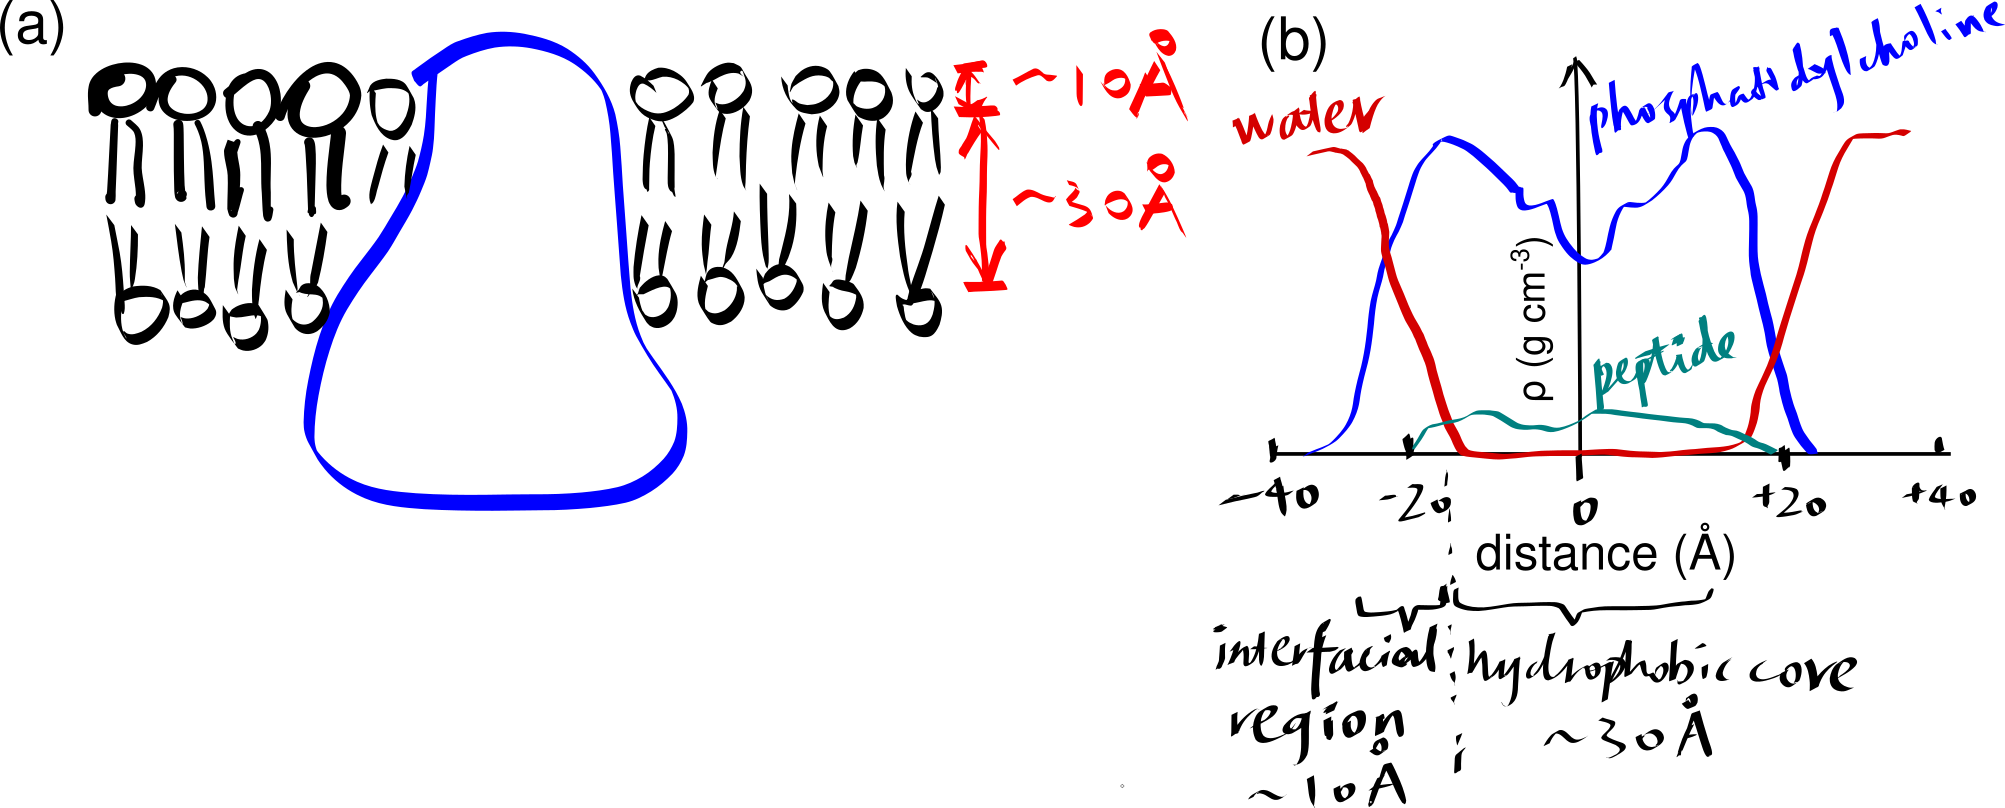
\includegraphics[width=1\linewidth]{../img/lipid-bilayer-diagram.png} \caption{(a)}\label{fig:lipid-bilayer-diagram}
\end{figure}

How many aa do
Thickness 30 angstroms

each residue corresponds to a translation of 1.5 angstroms along the axis of the helix
==\textgreater{} 20 aa in a row --\textgreater{} to form the 30 A helix to span the membrane

occupied by the long alkyl chains of lipid tails

The hydrophobic core region has a dielectric constant (\(\epsilon_{r}\)) of about 2, which is much lower than \(\epsilon_{r}\) of water (about 80), which means the same pair of charges separated by the same distance experience more electrostatic force in the membrane core than in water, according to the Coulomb's law:

\[F = \dfrac{q_1 q_2}{4\pi \epsilon_0 \epsilon_r r^2}\]

This has several implications on acidic and basic amino acid residues. First, the carboxyl group of acidic side chains are more difficult to dissociate (i.e.~p\(K_a\)s are shifted up), meaning they tend to remain in the uncharged (--COOH) form. Second, in \(\alpha\)-helical bundles, oppositely charged residues in adjacent helices associated more strongly than they do in aqueous environment. Third, this facilitates the snorkelling of lysine and arginine residues near the interface (Section \ref{snorkel}).

\hypertarget{amino-acids-at-the-hydrophobic-core-region}{%
\section{Amino Acids at the Hydrophobic Core Region}\label{amino-acids-at-the-hydrophobic-core-region}}

The transmembrane region of each helix in a \(\alpha\)-helical bundle is composed predominantly of hydrophobic amino acid residues (Ala, Leu, Ile, Val, Phe), which can be explained by simple thermodynamic reasoning. The water molecules in the aqueous environment outside the membrane are capable of forming relatively strong dipole-dipole interactions and hydrogen bonds (H-bonds) with polar (including charged) amino acids, while the non-polar alkyl groups that occupy the hydrophobic core of the membrane can only provide weak van der Waals interactions. Thus, if a helix composed mainly of polar amino acid residues is inserted into the membrane, the loss of strong interactions with water will make this process very energetically unfavourable (very large \(\Delta G\)). On the contrary, if a hydrophobic helix were present in an aqueous environment, it would disrupt the dipole-dipole interactions and hydrogen bonding among water and other polar molecules. Thus, its insertion into the membrane is energetically favourable.

This property of transmembrane helices allows them to be predicted using a hydropathy plot, in which the average hydrophobicity index of a fixed number of consecutive residues (a ``window''), \(H(i)\), is plotted against the index (\(i\)) of the window, i.e.

\[H(i) = \sum_{i<j<i+k}h(a_j)/k\]

for \(1 < i < n - k\), where n is the length (number of residues) of the peptide, \(h(a_j)\) is the hydrophobicity index of the \(j\)-th amino acid residue and \(k\) is the window size.

Every peak in the plot represents a highly hydrophobic local region in the peptide and thus indicates a potential transmembrane helix.

A small number of polar (even charged) residues within a TM helix can be tolerated as long as the overall transmembrane segment is hydrophobic enough. In addition, in polytopic proteins, polar residues in adjacent helices may help to stabilise each other. These non-hydrophobic residues often have special roles, as exemplified by voltage-gated K\textsuperscript{+}, Na\textsuperscript{+} and Ca\textsuperscript{2+} channels (K\textsubscript{v}/Na\textsubscript{v}/Ca\textsubscript{v}).

\hypertarget{glycine-and-proline-in-tm-helices}{%
\section{Glycine and Proline in TM Helices}\label{glycine-and-proline-in-tm-helices}}

The side chain of proline forms a pentameric ring with the amine group on the main chain. Thus, in a helix, the amine group of a proline does not have a hydrogen that can be H-bonded to the main chain C=O of the residue above it. This introduces local flexibility within a relatively regid helix and often forms a hinge. Similarly, due to glycine's small size, it can tolerate a much wider range of dihedral angles than other amino acids, which also makes it able to introduce flexibility.

Glycine and proline residues often introduce kinks or hinges in TM helices, due to

\hypertarget{most-integral-proteins-are-either-alpha-helical-bundle-or-beta-barrel}{%
\section{\texorpdfstring{Most integral proteins are either \(\alpha\)-helical bundle or \(\beta-barrel\)}{Most integral proteins are either \textbackslash alpha-helical bundle or \textbackslash beta-barrel}}\label{most-integral-proteins-are-either-alpha-helical-bundle-or-beta-barrel}}

\hypertarget{primary-structure}{%
\section{Primary Structure}\label{primary-structure}}

\hypertarget{snorkel}{%
\subsection{Tryptophan and Tyrosine at the Interface and Lysine/Arginine Snorkelling}\label{snorkel}}

\hypertarget{proline-and-glycine-in-alpha-helices}{%
\subsection{\texorpdfstring{Proline and Glycine in \(\alpha\)-helices}{Proline and Glycine in \textbackslash alpha-helices}}\label{proline-and-glycine-in-alpha-helices}}

KcsA, Kv1.2

Distortions allow for greater variability of the geometry of the transmembrane domains
also, flexibility

\hypertarget{tranmembrane-helix-insersion}{%
\subsection{Tranmembrane Helix Insersion}\label{tranmembrane-helix-insersion}}

in vitro basis:

if have a helix --\textgreater{} in the presence of bilayer --\textgreater{} partition from water to the bilaryer --\textgreater{} form a stable, TM Helix

in vivo:

translocaon SecY form s pore --\textgreater{} ejected laterally

Bowie 2005 Nature 438, 581

\hypertarget{membrane-protein-architectures}{%
\subsection{Membrane Protein Architectures}\label{membrane-protein-architectures}}

\(\alpha\)-helix bundles - predominant Architecture for membrane proteins: GlpF, KcsA
\(\beta\)-barrels--baterial outer membrane proteins OmpA (pore/structural protein)

\hypertarget{why-alpha-helix-stable}{%
\subsubsection{\texorpdfstring{Why \(\alpha\)-helix stable?}{Why \textbackslash alpha-helix stable?}}\label{why-alpha-helix-stable}}

Polar residues are not completely excluded from the transmembrane region

\hypertarget{interactions-with-lipids}{%
\section{Interactions with Lipids}\label{interactions-with-lipids}}

X-ray cyrstal structures cna reveal lipids that are strongly bound to membrane proteins (not removed by detergents).

cardiolipin to photosynthetic reaction centre

annular lipids

\hypertarget{primary-structure-1}{%
\section{Primary Structure}\label{primary-structure-1}}

\hypertarget{conclusion}{%
\section{Conclusion}\label{conclusion}}

\end{document}
